% This work is licensed under the Creative Commons
% Attribution-NonCommercial 3.0 Unported License. To view a copy of this
% license, visit http://creativecommons.org/licenses/by-nc/3.0/.

\section{Versuchsaufbau und Durchführung}

Zum Versuch werden verschiedene Meßgeräte, einige Abschlußwiderstände
und die zu untersuchenden Koaxialkabel selbst benötigt.  Dazu stehen
vier verschiedene Koaxialkabel zur Verfügung.  Jeder Versuchsabschnitt
ist im wesentlichen aus drei Komponenten aufgebaut: Meßgerät,
Signalgenerator und zu messendes Kabel.

\subsection{Bestimmung der Kabellänge}

Um die Länge eines Kabels zu bestimmen, wird ein Spannungspuls auf das
Kabel gegeben und dann mithilfe eines Oszilloskops die Zeitdifferenz
zwischen einlaufendem und reflektiertem Signal bestimmt.  Da sich das
Signal innerhalb der Leitung mit der Ausbreitungsgeschwindigkeit $c =
c_0/\sqrt{\epsilon_\text{r}}$ bewegt, gilt für die Länge des Kabels
daher:
% 
\begin{equation}
  \label{eq:laenge}
  L = c \frac{\Delta t}{2} = \frac{c_0 \Delta t}{2 \sqrt{\epsilon_\text{r}}}.
\end{equation}

\subsection{Bestimmung der Leitungskonstanten}

Zur Bestimmung der Leitungskonstanten wird das zu vermessene Kabel an
das RLC-Meßgerät angeschlossen, welches automatisch die Art des
Abschlußwiderstands erkennt und die entsprechenden Impedanzen anzeigt.

\subsection{Bestimmung des Dämpfungsbelags}

Zur Bestimmung des Dämpfungsbelags wird ein Rechteckpuls durch ein
kurzes Kabel an einen Spektrumsanalysator geschickt und dort mithilfe
einer \textit{Fast Fourier Transform} spektral analysiert.  Für das
kurze Kabel wird keine Dämpfung angenommen und die Amplituden der ersten
Oberwellen werden notiert.

Für ein zweites längeres Kabel wird dieselbe Prozedur durchgeführt und
die so erhaltenen Amplituden mit denjenigen, die mit kurzen Kabel
erhalten worden sind, verglichen.

\subsection{Mehrfachreflexion}
\label{sec:durchfuehrung-mehrfachreflexion}

In diesem Versuchsteil werden zwei unterschiedliche Koaxialkabel
(\SI{50}{\ohm} und \SI{75}{\ohm}) miteinander verbunden und ein
Spannungspuls auf das Kabel gegeben.  Die Leitung darf nicht angepaßt
sein, da es sonst zu keiner Reflexion kommt, welche hier beobachtet
werden soll, aber außer dem kann der Abschluß beliebig sein.

Wie bereits im Abschnitt über Mehrfachreflexion aus dem Theorieteil
beschrieben, kommt es innerhalb des Kabels zu mehreren Reflexionen
sowohl an Kabelanfang und -ende, als auch an der Verbindungsstelle der
Kabel.  Ein Impulsfahrplan ist in Abbildung~\ref{fig:impulsfahrplan} zu
sehen.

\begin{figure}
  \centering
  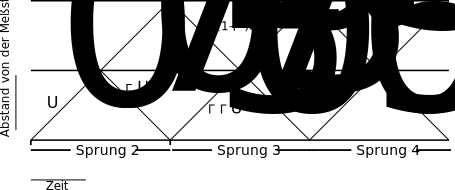
\includegraphics[width=0.8\textwidth]{impulsfahrplan}
  \caption{Der Impulsfahrplan für die Mehrfachreflexion des Signals, der
    sich aus der Verbindung zweier Koaxialkabel (\SI{50}{\ohm} und
    \SI{75}{\ohm}) ergibt.}
  \label{fig:impulsfahrplan}
\end{figure}

\subsection{Untersuchung der Abschlußwiderstände}

Der letzte Teil des Versuchs besteht in der Untersuchung unbekannter
Abschlußwiderstände.  Es wird ein Spannungspuls auf ein Kabel gegeben
und der zeitliche Signalverlauf auf dem Oszilloskop betrachtet.  Aus der
Form des Verlaufs können Rückschlüsse auf die Art der des
Abschlußwiderstandes gezogen werden und die Zeitkonstanten bestimmt
werden.
